%%
%% This is file `tikzposter-example.tex',
%% generated with the docstrip utility.
%%
%% The original source files were:
%%
%% tikzposter.dtx  (with options: `tikzposter-example.tex')
%% 
%% This is a generated file.
%% 
%% Copyright (C) 2014 by Pascal Richter, Elena Botoeva, Richard Barnard, and Dirk Surmann
%% 
%% This file may be distributed and/or modified under the
%% conditions of the LaTeX Project Public License, either
%% version 2.0 of this license or (at your option) any later
%% version. The latest version of this license is in:
%% 
%% http://www.latex-project.org/lppl.txt
%% 
%% and version 2.0 or later is part of all distributions of
%% LaTeX version 2013/12/01 or later.
%% 




 \documentclass[25pt, a0paper, portrait, margin=0mm, innermargin=15mm,
     blockverticalspace=15mm, colspace=15mm, subcolspace=8mm]{tikzposter} %Default values for poster format options.

 \tikzposterlatexaffectionproofon %shows small comment on how the poster was made at bottom of poster
\usepackage{graphicx}
 % Commands
 \newcommand{\bs}{\textbackslash}   % backslash
 \newcommand{\cmd}[1]{{\bf \color{red}#1}}   % highlights command

 % Title, Author, Institute
 \title{CODE-RADE}
 \author{Sean Murray, \& Bruce Becker}
 \institute{Council for Scientific and Industrial Research, Meraka. University of Cape Town}
\titlegraphic{img/coderade.png}

 % -- PREDEFINED THEMES ---------------------- %
 % Choose LAYOUT:  Default, Basic, Rays, Simple, Envelope, Wave, Board, Autumn, Desert,
\usetheme{Rays} % Board, Simple, Wave, Rays.
\usecolorstyle[colorPalette=BrownBlueOrange]{Envelope}


 \begin{document}

     \maketitle{}
% basic structure
% Summary of arch and tech
% schematic of code-rade workflow, the actors etc.
% diagram of delivery 
     % map of whereit can be run (grid sites)
% description of repos and repo layouts.
% todo and next features

     \begin{columns}%blocks will be placed into columns
         \column{.5}
         \block[roundedcorners=40]{The problem solved by CODE-RADE}{
             \begin{itemize}
                 \item Lowers barrier to entry to grid or cloud infrastructure, or a single HPC site.
                 \item Application expert can prove to resource provider that the application will run on the sites execution environment
                 \item Easily manages the lifecycle of applications across multiple versions, architectures and configurations
                 \item Ensures that once an application is certified, its available on as many sites as possible.
                 \item Promotes collaboration between researcher, research software engineer, and infrastructure provider.
             \end{itemize}
        }
%         \block[roundedcorners=40]{7 Hypotheses of scientific computing}{
%             \begin{itemize}
%                 \item It always comes down to an application
%                 \item No software is an island
%                 \item Applications require environments.
%                 \item There are multiple environments
%                 \item Solutions decay 
%                 \item Remove humans
%                 \item Stuff is not hard, leverage what is around
%
%             \end{itemize}
%         }

         \block[roundedcorners=40]{Achitecture}{
             \begin{itemize}
                     \item CODE-RADE Components
                           \begin{itemize}
                               \item Version Control (Github)
                               \item Continuous Integration (Jenkins)
                               \item Automated Delivery (CVMFS)
                           \end{itemize}
                     \item CODE-RADE workflow 
                         \begin{itemize}
                                 \item Build : User/expert-defined means to produce executable applications or libraries
                                 \item Test : Infrastructure operator-defined targets means to ensure viability
                                 \item Deliver : Ensure once tests pass, the application is available.
                         \end{itemize}
             \end{itemize}

         }
         \column{0.5}
         \block[roundedcorners=40]{Technology}{
             \begin{itemize}
                 \item docker
                 \item quay.io
                 \item persistant storage
                 \item R
                 \item S
             \end{itemize}
        }
     \end{columns}

     \block[bodyoffsety=-1cm]{CODE-RADE Work Flow}{\vspace{2em}
     %\block[titleoffsety=-1cm,bodyoffsety=-1cm]{Sample document}{\vspace{2em}
   % \includegraphics{img/sagrid.png} 
    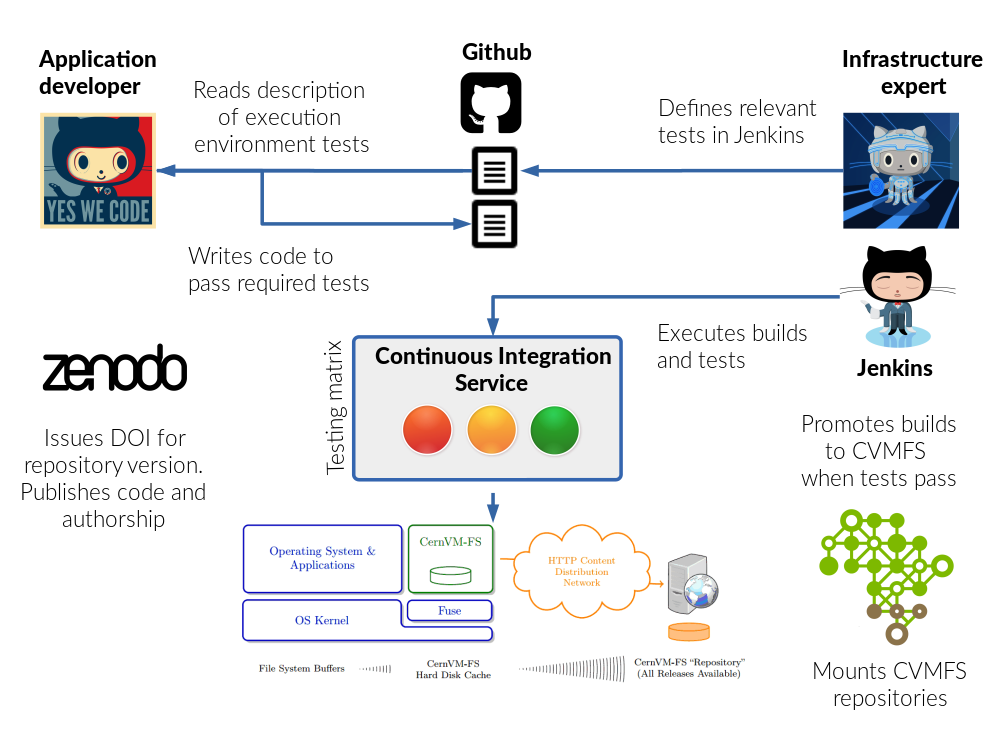
\includegraphics[scale=0.7]{img/Jenkinsworkflowschematic.png} 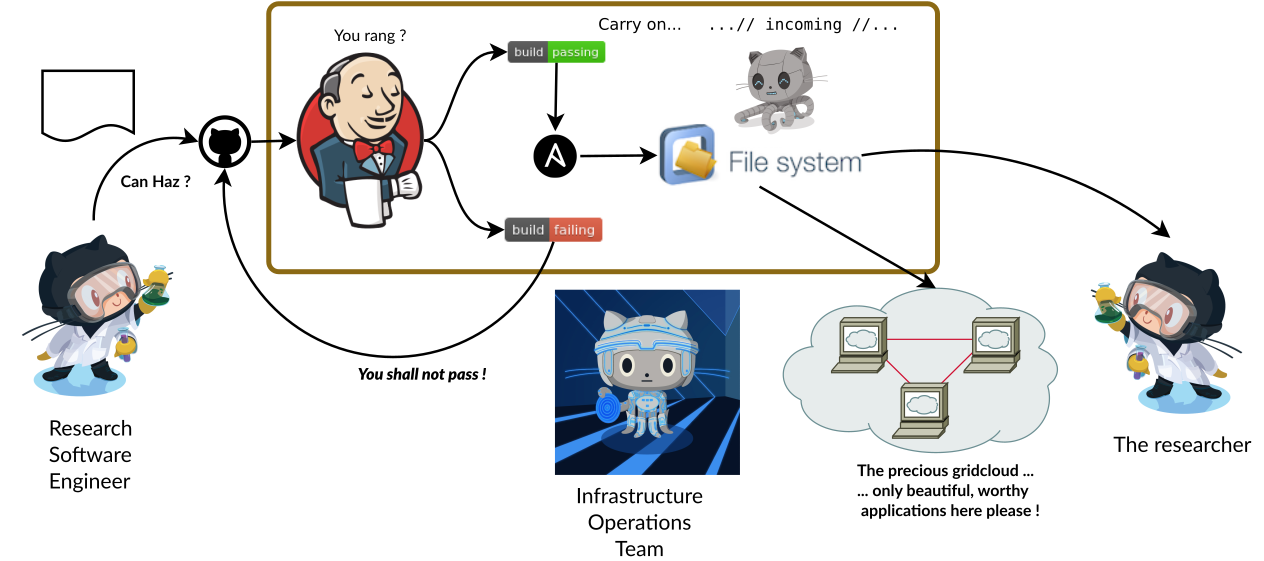
\includegraphics[scale=1.25]{img/code-rade-jenkins-magic.png}
     }
     % map of whereit can be run (grid sites)
% description of repos and repo layouts.
% todo and next features

     \begin{columns}%blocks will be placed into columns
         \column{.5}
         \block[roundedcorners=40]{Where can all this can run}{
             %  \includegraphics{}
         }

         \column{0.5}
         \block[roundedcorners=40]{Repositories}{
             \begin{itemize}
                 \item I
             \end{itemize}
        }
         \block[roundedcorners=40]{Repository Layout}{
             \begin{itemize}
                 \item R
             \end{itemize}
        }
         \block[roundedcorners=40]{Where to from here}{
             \begin{itemize}
                 \item R
             \end{itemize}
        }
     \end{columns}
     
     \block[bodyoffsety=-1cm]{Acknowledgements}{\vspace{2em}
     %\block[titleoffsety=-1cm,bodyoffsety=-1cm]{Sample document}{\vspace{2em}
   
\includegraphics{img/coderade.png}  
   \center Feedback and discussion at discourse.sci-gaia.eu
   \begin{flushright}
\includegraphics[scale=0.25]{img/SANCG_logoTransparent-cropped.png}\end{flushright}
     }

 \end{document}




\endinput
%%
%% End of file `tikzposter-example.tex'.
